\section{Deep Reinforcement Learning}
\label{sec:rl}
In contrast to the manually developed algorithms, a Deep Q-learning approach as also explored. The agents are trained using the simple simulator. Reinforcement learning suits this problem well, as coverage can serve as a reward function. Traditional Q-learning methods store a table of discrete state-action pairs and their expected reward in memory {\color{red}[SOURCE]}, which can be cumbersome in real world applications where state is often continuous. Another pitfall of traditional Q-learning is that the size of the Q-table grows with the state space. Neural networks solve both of these problems. The Q-table can be approximated by using a neural network, then used to pick an action given a state. This is network is called a DQN (Deep Q Network). \\

Designing a neural network involves several important considerations, including selecting the number of layers and neurons, choosing appropriate activation functions, and determining key hyperparameters such as the learning rate. After the architecture is defined, the network must be trained, evaluated, and iteratively optimized to ensure stable and effective learning. Finally, the trained model can be validated on unseen environments and integrated into the broader system for deployment.

% TODO: How much should we explain neural networks and Q-learning?
\subsection{Network}
The general idea of a neural network is to construct a layered architecture where each layer, consists of multiple interconnected neurons. Each neuron applies a learned weight and bias to its inputs and passes the result through an activation function. The final output of the network determines the action that the agent should take based on the current input state.

\subsection{Learning Framework}
The framework for defining robots controlled by neural networks is implemented as a part of the \texttt{botbrain} library and can be enabled by the "rl" feature flag. The models are implemented using the \texttt{burn} \cite{burn} library, which is a Rust Deep Learning Framework. \texttt{burn} provides a high-level API for building and training deep learning networks with multiple backends. \\

\texttt{botbrain} defines the \texttt{RlRobot} which is generic across four parameters: the \texttt{burn} backend, the state type which the robots provides as input to the network, the action type which defines the discrete actions the robot can take, and the network which defined how the input and output layers should be connected. Several state, action and network implementations are also provided, which can be combined in any combination to create specializations of \texttt{RlRobot}. This system facilitates composition and expansion the \texttt{RlRobot} state and makes it easy to swap out single elements and compare differing architectures.

% TODO: Maybe create a figure

% over the network architecture within \texttt{RlRobot} and makes is possible to compare robots.


% TODO: Write how our network and activation function works (maybe in each of the models or only one?)
% For this project, a feedforward fully connected neural network was used. The input to the network is a tensor representation part of the robot’s state, including sensor readings, and proximity to other robots. 

% The output tensor represents descrete set of actions the robot can take. This is different values of steer angle and speed for the TurtleBot 4.

% The network also consists of two hidden layers, with varying sizes depending on the model, and uses the ReLU (Rectified Linear Unit) activation function for all hidden layers.

\subsection{Reward}
The reward function is a central component of reinforcement learning, as it defines the value of agent actions. A well designed reward function encourages desirable behavior and penalizes undesirable outcomes. \\

In this project, the reward is primarily based on map coverage. At each time step, a positive reward is given proportional to the amount of new area explored by the agent. This incentivizes the agent to move into unexplored regions of the map. Additionally, a small negative reward is applied for each step to encourage efficiency and to discourage the agent from idling or circling already explored areas. This negative also scales linearly with the time since new area was covered. A further negative reward is given when the robot collides a wall to promote safe navigation.
% TODO: Correct if we did not use negative reward for range
% TODO: Actually implement negative reward outside of range
To maintain network connectivity among robots, a penalty is also introduced if the agent moves outside of the communication range of the rest of the swarm. This helps keep the robots together to allow them to communicate.

% TODO: Write this section
\subsection{Target and Policy Networks}

\subsection{Training}
Training the neural network involves allowing the agent to interact with the environment over multiple episodes while incrementally improving its policy based on received rewards. The \texttt{trainer} is implemented as a seperate program and was inspired by the \texttt{burn-rl-examples} repository \cite{burn-rl-examples}. \\

Each training episode starts with one or more robots placed in a randomly generated environment, as described in the next subsection {\color{red}DESCRIBE?}. The episode proceeds step by step, during which the agent observes its current state, selects an action using an $\epsilon$-greedy policy, balancing exploration and exploitation, executes the action, and receives a reward. The transition tuple,  containing state, action, reward and next state, is stored in a replay buffer. \\

Each time step, mini-batches of transitions are sampled randomly from the replay buffer and used to train the policy network by performing gradient decent on the loss function. Loss is calculated as the mean square error of the state-action-values, as infered by the policy network, and the target state-action values as calculated by the 

% $$Q_{\text{target}} = r_t + \gamma \max_{a'} Q(s_{t+1}, a')$$
% where $\gamma$ is the discount factor.\\

Training continues for a fixed number of episodes or until the performance converges. An episode is terminated early if the agent fails to make significant progress (i.e., no new area is explored for a defined number of steps), or when the entire map is successfully covered.


\subsubsection{Generating Training Environments}
As to not overfit the network, it must be trained on many different environments. A simple program was created to generate worlds populated by line and circle obstacles.

% The use of randomly generated maps with varying obstacle layouts (see Fig.~\ref{fig:generated-enviornments}) ensures that the agent generalizes its behavior across diverse spatial configurations, rather than overfitting to a single scenario.

\def\w{0.31\textwidth}
\begin{figure}[H]
    \begin{subfigure}{\w}
        \makebox(\textwidth, \textwidth)[\textwidth]{
            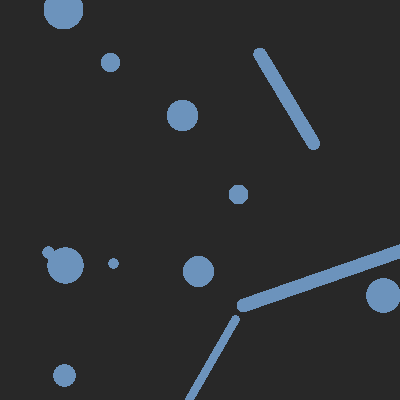
\includegraphics[width=\linewidth]{figures/generated-worlds/world_0.png}
        }
    \end{subfigure}
    \hspace*{\fill}
    \begin{subfigure}{\w}
        \makebox(\textwidth, \textwidth)[\textwidth]{
            
\includegraphics[width=\linewidth]{figures/generated-worlds/world_1.png}
        }
    \end{subfigure}
    \hspace*{\fill}
    \begin{subfigure}{\w}
        \makebox(\textwidth, \textwidth)[\textwidth]{
            
\includegraphics[width=\linewidth]{figures/generated-worlds/world_2.png}
        }
    \end{subfigure}

    \vspace{4mm}

    \begin{subfigure}{\w}
        \makebox(\textwidth, \textwidth)[\textwidth]{
            
\includegraphics[width=\linewidth]{figures/generated-worlds/world_3.png}
        }
    \end{subfigure}
    \hspace*{\fill}
    \begin{subfigure}{\w}
        \makebox(\textwidth, \textwidth)[\textwidth]{
            
\includegraphics[width=\linewidth]{figures/generated-worlds/world_4.png}
        }
    \end{subfigure}
    \hspace*{\fill}
    \begin{subfigure}{\w}
        \makebox(\textwidth, \textwidth)[\textwidth]{
            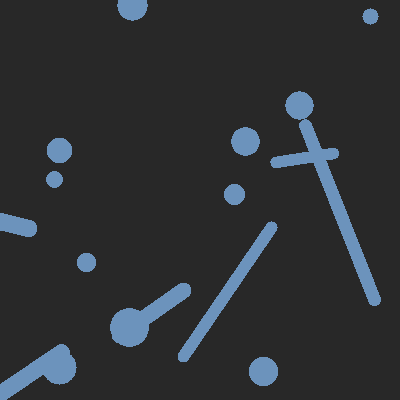
\includegraphics[width=\linewidth]{figures/generated-worlds/world_5.png}
        }
    \end{subfigure}
    \caption{Examples of generated environments} \label{fig:generated-enviornments}
\end{figure}


% TODO: If better hardware how could we train it better?
% How is the params, (maybe better to look at than pure performance)
% Why is it not that good?
%   Leaning rate?
%   Cost function?
